\documentclass{article} % For LaTeX2e
\usepackage{nips13submit_e,times}
\usepackage{hyperref}
\usepackage{url}
\usepackage{amsmath}
\usepackage{graphicx}

%\documentstyle[nips13submit_09,times,art10]{article} % For LaTeX 2.09


\title{Migration Network Inference with eBird}

\author{
Casey Battaglino \\
Georgia Institute of Technology\\
Atlanta, GA 30332 \\
\texttt{cbattaglino3@gatech.edu} \\
\And
Robert Pienta \\
Georgia Institute of Technology \\
Atlanta, GA 30332 \\
\texttt{pientars@gatech.edu} \\
}

% The \author macro works with any number of authors. There are two commands
% used to separate the names and addresses of multiple authors: \And and \AND.
%
% Using \And between authors leaves it to \LaTeX{} to determine where to break
% the lines. Using \AND forces a linebreak at that point. So, if \LaTeX{}
% puts 3 of 4 authors names on the first line, and the last on the second
% line, try using \AND instead of \And before the third author name.

\newcommand{\fix}{\marginpar{FIX}}
\newcommand{\new}{\marginpar{NEW}}

\nipsfinalcopy % Uncomment for camera-ready version

\begin{document}
\maketitle

\begin{abstract}
eBird is a citizen science application that employs a statistical model to predict the spatial and temporal distribution of bird species throughout the United States. However, they do not offer a migration model. We discuss the process of `network inference,' initially developed to discover implicit networks in the brain from time-series data. We then discuss how we efficiently adapt this process to bird presence data, and analyze its suitability for detecting bird migration networks. 
\end{abstract}

\section{Introduction}
eBird\cite{DBLP:conf/iaai/KellingGFLWYDG12} is a `citizen science' project that allows for users to report and store bird sightings online. This allows for the crowd-sourcing of bird identification and monitoring, a process that would otherwise require massive amounts of time and effort from researchers. 

While this removes the burden of data collection from experts, it also introduces a number of new problems. In particular, it introduces a higher probability of misidentification (when non-experts attempt to identify birds), and introduces spatial bias, concentrating results around areas of high human population. Thus, data must be sanitized and normalized before it can be used to actually model bird presence. Implemented solutions to these issues are presented in Kelling, et. al~\cite{DBLP:conf/iaai/KellingGFLWYDG12}.

The problem of generating spatially and temporally continuous species distribution from this data is discussed in the `STEM' paper of Fink, et. al~\cite{stem}. We are interested in using the output of this model to explore higher-level questions regarding the movement of migratory birds. In particular, we are interested in inferring an underlying migration network of a given species, given its spatial distribution over time. In our proposed model, nodes in the network represent a contiguous area of the United States, and weighted edges in the network represent the likelihood of bird migration from location to location. 

\begin{figure}[h!]
\centering
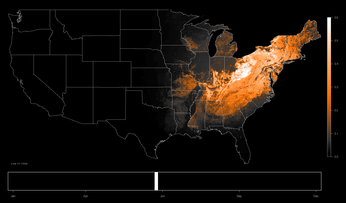
\includegraphics[scale=0.65] {stem}
\caption[Caption for]{Example of STEM output (\url{http://ebird.org/content/ebird/occurrence/})}
\label{fig:00}
\end{figure}

\section{Motivation}
Human development can infringe upon important bird habitats, reducing biodiversity. In particular, there is evidence that migratory birds are less likely to inhabit areas of increasing human development~\cite{riparian}. Thus, to minimize disruption of migration, we should be aware of prominent migration corridors so that we can prioritize them in conservation efforts. The 'sources' and 'sinks' of this network are also key candidates for conservation efforts.

As a crowd-sourced research project, eBird presents a more horizontal data collection effort: instead of creating a model built from a small number of researchers' observations, we can aggregate data from thousands of observers around the United States. While this creates unique challenges due to spatial bias and inexperienced observers, it also allows for much larger statistical data sets to draw from. 

Creating a migration model based on eBird data theoretically allows us to study \textit{real-time}, \textit{crowd-sourced} temporal migration patterns, rather than static models aggregated over many years. This gives us the additional potential to see changes in migration patterns on a smaller, more agile time scale.

\section{Data}
Our approach relies on the availability of clean, reliable data for bird distribution from eBird. Through correspondence with Prof. Dilikina, we acquired access to spatio-temporal data for two species of migratory birds, generated by the STEM model~\cite{stem}. 

This data provides a time-series of estimated bird presence for roughly one million points distributed through the United States. Each time-series is divided into fifty-two points within the year of 2011, or roughly one data point per week. Our model reduces noise and computational complexity by aggregating this data into a smaller number of coarse points, regularly distributed through the US. 


\subsection{Transformation}
Our first step was to aggregate the one million data points to a more manageable number. We divided the coordinate grid of the United states into $2500 (50 \times 50)$ bounding boxes. We then aggregated all time series within each bounding box to generate an average. The geographical center of each bounding box then provided the coordinates for the generated node in our network. 

Our goal is network inference --- we wish to select a network that represents bird migration through these points in a given time slice, from all possible candidate edges. In the naive case, we would have to compare the time series data between every two points, for a total of $2500^2 = O(n^2)$ time-series comparisons Fortunately, we only care about constructing a network that joins nodes that are geographically close (because it is infeasible for birds to instantly travel large distances). Thus, we construct an overlay network out of the nodes where any two nodes within a certain geographical distance are connected by an edge --- the presence of an edge in this overlay network means that we will consider it as a candidate for network inference, and perform a correlation computation between the two nodes. Because this overlay network is planar, we only need to make $O(n)$ time-series comparisons (provided our `closeness' criteria is a small function of our `coarseness' criteria). In practice, we restricted the comparisons to the `8-neighborhood' of each node. This particular distance would be a tuning variable in a theoretical future model, given that different birds travel at different speed. 

\begin{figure}[h!]
\centering
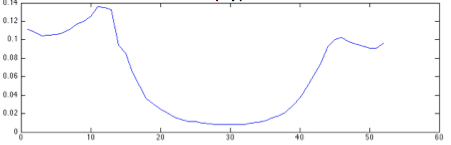
\includegraphics[scale=0.65] {ts}
\caption[Caption for]{Example of a single STEM time-series, averaged from all nearby locations}
\label{fig:00}
\end{figure}

\section{Network Inference} 
The statistical approach to graph inference is a well researched area with existing effective techniques \cite{AlbertMechanics}. Because the nature of this research problem involves inferring a network from a time-varying signal, we will leverage the work of Kramer et al. who proposed a state of the art method for statistically inferring an underlying functional network from a time-varied signal~\cite{kramer}. In this case, we attempt to establish the existence of signal propagation from one node to another, with a certain degree of confidence. 

Kramer, et. al present three methods of increasing sophistication (and increasing computational intensity) for inferring a network from a set of nodes and corresponding time-series data. The final, most sophisticated method is computationally infeasible for large data sets (requiring a massive number of FFTs compounded by a massive number of bootstrap runs), so we explore the effectiveness of the initial two methods in our work. 

Network inference generally takes three steps~\cite{kramer}:
\begin{enumerate}
\item Define a coupling measure between pairs of nodes (i.e, cross-correlation)
\item Utilize a significance test to detect statistically significant couplings
\item Integrate with further significance tests, if necessary
\end{enumerate}

In the approach taken by Kramer, et. al, the coupling measure is cross correlation:

\[ C_{ij}[\tau] = \frac{1}{\hat\sigma_i\hat\sigma_j (n-2\tau)}\sum_{t=1}^{n-\tau}(x_i[t] - \bar x_i )(x_j[t+\tau] - \bar x_j) \]

The extrema from this correlation will likely be produced in such a way that normal-based significance tests will fail. Thus, we compute new values using the Fisher transformation, which we then perform a significance test on:

\[ C_{ij}^F [\tau] = \frac{1}{2} \ln \frac{1+C_{ij}[\tau]}{1-C_{ij}[\tau]} \]

A final detail is that we will need to look at `slices' of the time-series data and perform network inference for a set number of time periods (to account for different migratory behaviors in different seasons). The final network can be unweighted (where an edge exists if its weight is above a certain threshold), or weighted by the confidence that it is in the migratory network, to identify important corridors, sources, and sinks using a flow analysis. 

As mentioned above, we avoid looking at all possible $n \choose 2$ edges by only looking at the 8-neighborhood of each node, for a total number of correlation computations of $8n$.

\section{Implementation}
The STEM data produced by eBird came in \texttt{Rdata} format. Thus, our first step is transforming that data into CSV format. We then read the data into Python where we generate the averaged time-series data for each bounding box (with the number of boxes as a parameter). 

Our network inference implementation then chooses a time-window of roughly 2 months and computes the cross-correlation for all candidate edges (which are the $8n$ 8-neighborhood edges noted above, minus any with incident nodes that have been filtered due to low population). We then perform the Fisher transformation of the correlations, and perform the significance test. Thus, the general process is as follows:

\begin{enumerate}
\item Filter out zero-population and low-action ($p_{active} < 0.1$) nodes
\item Compute spatially localized cross-correlations with lags $1\dots T, (T=10)$
\item Use significance test to determine if cross-correlations are statistically valid
\item Keep valid edges
\end{enumerate}

The edges generated for each time period are returned as a list of tuples which can then be plotted on a map.

\section{Results}

\section{Conclusion}

\section{Future Work}
Qualitatively analyzing networks gives a limited picture. Quantitative measures can leverage the data more deeply. While betweenness centrality could identify some important `bottleneck' nodes, we believe that a maximum-flow measure would be more suitable, as this could also identify important sources and sinks if modeled correctly.

The most important future work, were this to become a publication, is validation of the produced data with well-known existing migration patterns, as well as further analysis with a wide spread of bird species.

\section{Related Work}
The data from eBird was already used by Hurlbert et al. in an investigation of red vireo migration; wherein they discovered a direct correlation between the migration patterns and the average temperature \cite{hurlbert}. 

Another migration study, using Hidden Markov models on synthetic data, was performed by Sheldon, et. al \cite{conf/nips/SheldonEK07}. 

\bibliographystyle{plain}
\bibliography{bib}

\end{document}